\chapter{Results}\label{chapter:results} \

In Chapter~\ref{chapter:results} we will introduce
the results of the experiments presented in Chapter
~\ref{chapter:implementation}. The results will be presented
per dataset. Each dataset contains two graphs related to
the model accuracy on the clean test set for noisy and
noiseless models. Additionally, two more graphs are
introduced to portray the effect of the adversarial
attacks on the noiseless \ac{qml} model, one for each
attack with increasing attack strengths. Finally, two
graphs for each of the six noise models are provided.
These last graphs will provide insights of the effects
of the diverse quantum noise sources with different noise 
magnitudes on the adversarial accuracy of both adversarial
attacks. \

In Section~\ref{section:iris-eval} the results from
the Iris dataset are shown. In Section~\ref{section:diabetes-eval}
the results from the \ac{pid} dataset follow. Moreover,
in Section~\ref{section:breast-cancer-eval} the outcomes
for the Wisconsin Breast Cancer dataset can be found.
Lastly, the experiments' outcomes from the Plus-Minus dataset
are provided in Section~\ref{section:plus-minus-eval}. \

\section{Iris Dataset}\label{section:iris-eval} \

The results obtained from training the noisy and noiseless
\ac{qml} models can be found in Subsection
~\ref{subsection:iris-noisy-acc}. Moreover, the outcomes
of both adversarial attacks will be presented in Subsection
~\ref{subsection:iris-adv-acc}. Finally, the evaluation
of the noisy models against the adverssarial attacks can
are presented in Subsection~\ref{subsection:iris-noisy-adv-acc}. \

\subsection{Noisy Models Accuracy}\label{subsection:iris-noisy-acc} \

In Figure~\ref{fig:iris-12} we can observe the results
from the training of noiseless and noisy \ac{qml} models
for the Iris test dataset. The noiseless baseline model accuracy
can be found on both graphs at the y-intercept, which in
this case is of \(100\%\). We note in Subfigure~\ref{fig:iris1}
that for the Iris dataset there are no perceptible
repercussions on the model accuracy when training with
coherent noise and remains the same as the noiseless
baseline performance. \

Nevertheless, for incoherent noise models in Subfigure
~\ref{fig:iris2} we can already observe a decrease in
model accuracy for certain noise models. For depolarizing
noise and bit-flip induced noise we notice the same behavior
as with coherent noise, remaining constant throughout
the different noise magnitudes and obtaining the same
performance as the noiseless model. \

Regarding phase damping noise, the model performance
marginally decreases the accuracy to \(97\%\) starting at
\(8\%\) noise probability. For phase-flip induced noise
the model performance slightly decreases in comparison
to phase damping noise to \(90\%\) at \(6\%\) noise probability
until the accuracy decreases to \(86\%\) at \(10\%\). Moreover,
for amplitude damping noise we can appreciate that the model
performance oscilates significantly starting \(4\%\) noise
probability. Furthermore, amplitude damping \ac{qml}
model's accuracy is significantly lower than other noiseless
and noisy models, reaching \(50\%\) accuracy at \(10\%\)
noise probability. \

\begin{figure}[!h]
  \centering

  \begin{subfigure}{0.45\textwidth}
      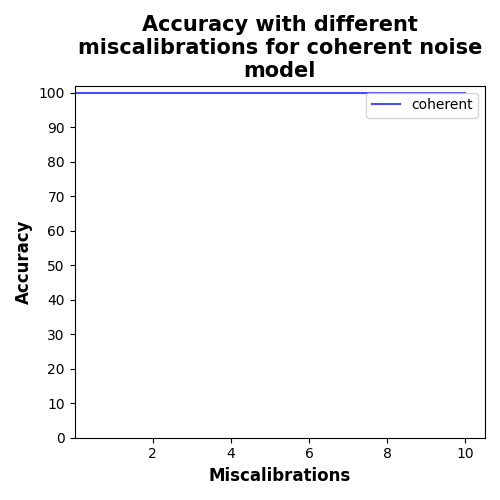
\includegraphics[width=\linewidth]{figures/evaluation_results/iris/pqc/figures/accuracy-coherent.png}
      \subcaption{Coherent noise model's accuracy.}
      \label{fig:iris1}
  \end{subfigure} \qquad
  \begin{subfigure}{0.45\textwidth}
      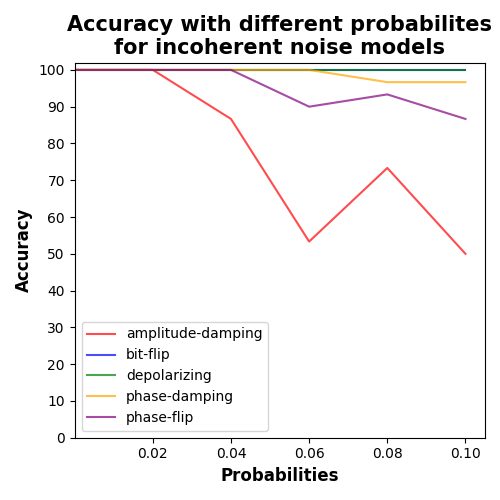
\includegraphics[width=\linewidth]{figures/evaluation_results/iris/pqc/figures/accuracy-incoherent.png}
      \subcaption{Incoherent noise models' accuracy.}
      \label{fig:iris2}
  \end{subfigure}

  \caption{\ac{vqa}'s accuracy on the Iris clean test dataset.}
  \label{fig:iris-12}
\end{figure} \

\subsection{Adversarial Accuracy}\label{subsection:iris-adv-acc} \

In Figure~\ref{fig:iris-34} we introduce the effects of the
adversarial attacks on the accuracy of the noiseless \ac{qml}
model. As expected, we can observe that for both adversarial
techniques the performance of the model decreases with increasing
attack strength. For the \ac{fgsm} technique in Subfigure~\ref{fig:iris3}
we notice a stark accuracy decrease until it stabilizes to around
\(50\%\) after \(0.5\) attack strength. Furthermore, in Subfigure
~\ref{fig:iris4} for the \ac{pgd} technique we see a lesser performance
decrease that stabilizes to around \(70\%\) after \(0.5\) attack strength. 
That \ac{fgsm} has a bigger performance impact than \ac{pgd} is expected
as \ac{fgsm}'s perturbations tend to be bigger in magnitude and more
disruptive to the input. \

\begin{figure}[!h]
  \centering

  \begin{subfigure}{0.45\textwidth}
      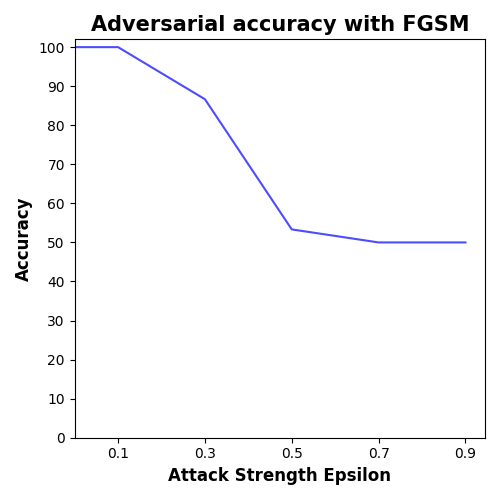
\includegraphics[width=\linewidth]{figures/evaluation_results/iris/pqc/figures/none-fgsm.png}
      \subcaption{Noiseless model's \ac{fgsm} adversarial accuracy.}
      \label{fig:iris3}
  \end{subfigure} \qquad
  \begin{subfigure}{0.45\textwidth}
      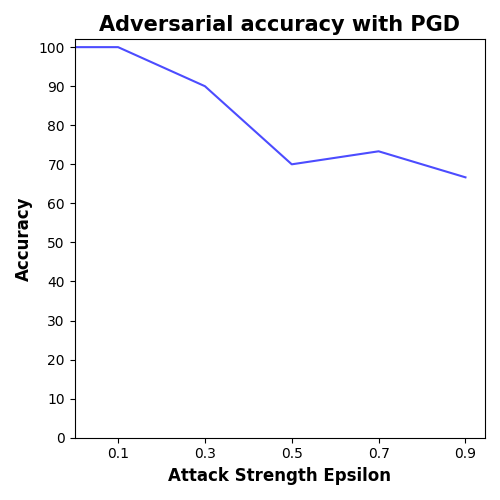
\includegraphics[width=\linewidth]{figures/evaluation_results/iris/pqc/figures/none-pgd.png}
      \subcaption{Noiseless model's \ac{pgd} adversarial accuracy.}
      \label{fig:iris4}
  \end{subfigure}

  \caption{\ac{vqa}'s accuracy on the adversarial Iris test dataset.}
  \label{fig:iris-34}
\end{figure} \

\subsection{Noisy Models Adversarial Accuracy}\label{subsection:iris-noisy-adv-acc} \

In this subsection we introduce the results from performing
the adversarial attacks on the noisy models with different noise
magnitudes for the Iris dataset. In each graph the color gray
represents the baseline adversarial accuracy obtained by the
noiseless model. \

In Figure~\ref{fig:iris-56} we present the outcomes from the amplitude
damping noisy models evaluation. For \ac{fgsm} in Subfigure~\ref{fig:iris5}
we note that the model with \(2\%\) noise probability obtains the same
performance as the noiseless model. Furthermore, we observe that an
increase in noise probability when training in general does not equate
to a worse adversarial accuracy at lower attack strengths, as the model
with \(8\%\) noise probability performs better than the one with \(6\%\)
noise probability. Nevertheless, once the attack strength reaches a
value of \(0.9\) all the models perform equally, converging to \(50\%\)
accuracy. \

\begin{figure}[!h]
  \centering

  \begin{subfigure}{0.45\textwidth}
      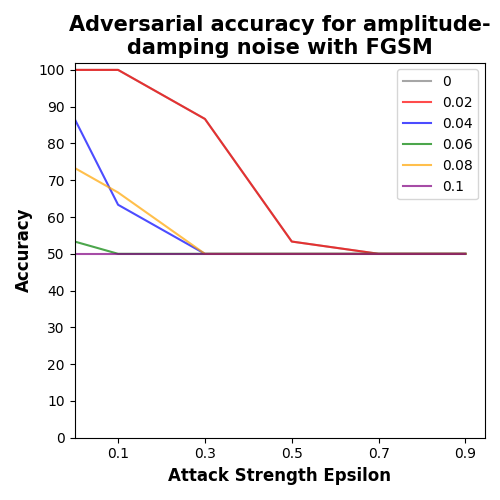
\includegraphics[width=\linewidth]{figures/evaluation_results/iris/pqc/figures/amplitude-damping-fgsm.png}
      \subcaption{Amplitude damping noise model's \ac{fgsm} adversarial accuracy.}
      \label{fig:iris5}
  \end{subfigure} \qquad
  \begin{subfigure}{0.45\textwidth}
      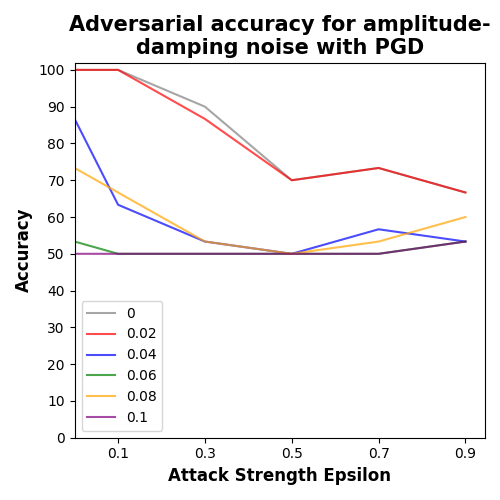
\includegraphics[width=\linewidth]{figures/evaluation_results/iris/pqc/figures/amplitude-damping-pgd.png}
      \subcaption{Amplitude damping noise model's \ac{pgd} adversarial accuracy.}
      \label{fig:iris6}
  \end{subfigure}
  \caption{Amplitude damping noise models' accuracy on the adversarial Iris test dataset.}
  \label{fig:iris-56}
\end{figure} \

In Subfigure~\ref{fig:iris6} we introduce the results from the \ac{pgd}
attack on the amplitude damping noisy models. As with the \ac{fgsm} attack
we can observe that the best performing model (close to the noiseless
model's performance) is the one with the smallest noise probability. Also,
we can note that increasing noise probability does not equal a direct
decrease in adversarial accuracy at lower attack strengths. Nevertheless,
noisy models in general perform significantly worse than the noiseless
model. Interestingly, when the attack strength surpasses \(0.5\), all
the noisy models (with the exception of the model with \(2\%\) noise
probability) perform slightly better than at lower attack strengths. \

In Figure~\ref{fig:iris-78} we present the outcomes from the bit-flip
noisy models evaluation. For \ac{fgsm} in Subfigure~\ref{fig:iris7}
we note that there are some models (\(2\%, 4\%, 10\%\)) performing
better than the noiseless model, while others (\(6\%, 8\%\)) have
a lower or equal adversarial accuracy throughout the different
attack strengths. While the model trained with \(10\%\) noise
probability performs the best against attack strength's lower
than \(0.7\), the adversarial accuracy drops to around \(33\%\)
(the lowest recorded accuracy) at an attack strenght of \(0.9\). \

\begin{figure}[!h]
  \centering

  \begin{subfigure}{0.45\textwidth}
      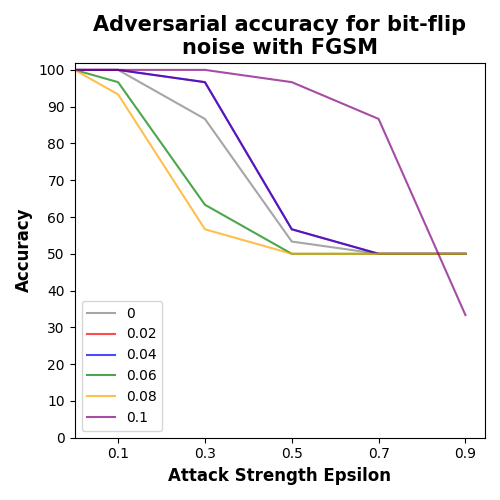
\includegraphics[width=\linewidth]{figures/evaluation_results/iris/pqc/figures/bit-flip-fgsm.png}
      \subcaption{Bit-Flip noise model's \ac{fgsm} adversarial accuracy.}
      \label{fig:iris7}
  \end{subfigure} \qquad
  \begin{subfigure}{0.45\textwidth}
      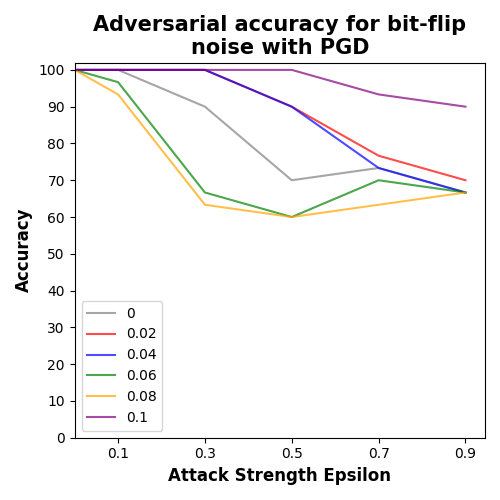
\includegraphics[width=\linewidth]{figures/evaluation_results/iris/pqc/figures/bit-flip-pgd.png}
      \subcaption{Bit-Flip noise model's \ac{pgd} adversarial accuracy.}
      \label{fig:iris8}
  \end{subfigure}
  \caption{Bit-Flip noise models' accuracy on the adversarial Iris test dataset.}
  \label{fig:iris-78}
\end{figure} \

In Subfigure~\ref{fig:iris8} we introduce the results from the \ac{pgd}
attack on the amplitude damping noisy models. \

\begin{figure}[!h]
  \centering

  \begin{subfigure}{0.45\textwidth}
      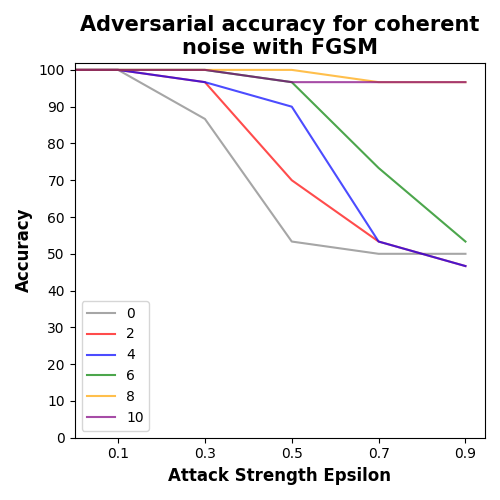
\includegraphics[width=\linewidth]{figures/evaluation_results/iris/pqc/figures/coherent-fgsm.png}
      \subcaption{Coherent noise model's \ac{fgsm} adversarial accuracy.}
      \label{fig:iris9}
  \end{subfigure} \qquad
  \begin{subfigure}{0.45\textwidth}
      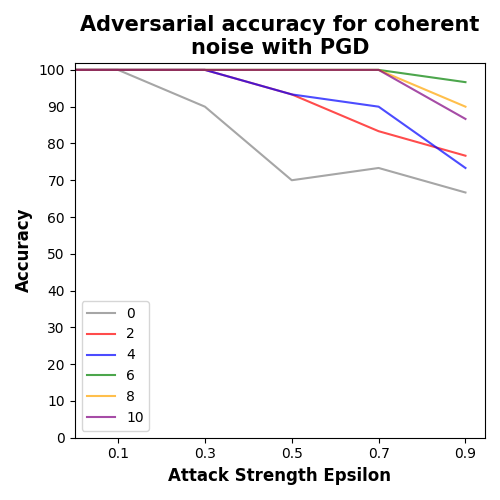
\includegraphics[width=\linewidth]{figures/evaluation_results/iris/pqc/figures/coherent-pgd.png}
      \subcaption{Coherent noise model's \ac{pgd} adversarial accuracy.}
      \label{fig:iris10}
  \end{subfigure}
  \caption{Coherent noise models' accuracy on the adversarial Iris test dataset.}
  \label{fig:iris-910}
\end{figure} \

\begin{figure}[!h]
  \centering

  \begin{subfigure}{0.45\textwidth}
      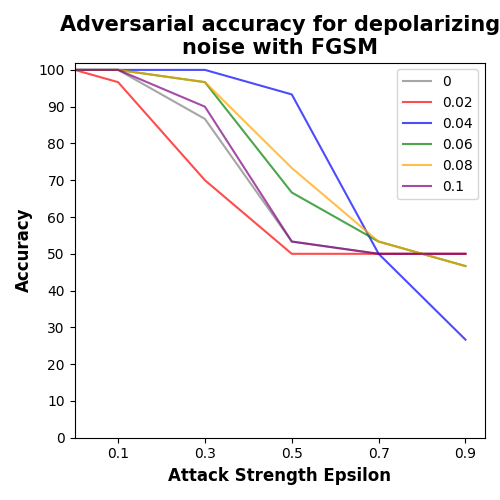
\includegraphics[width=\linewidth]{figures/evaluation_results/iris/pqc/figures/depolarizing-fgsm.png}
      \subcaption{Depolarizing noise model's \ac{fgsm} adversarial accuracy.}
      \label{fig:iris11}
  \end{subfigure} \qquad
  \begin{subfigure}{0.45\textwidth}
      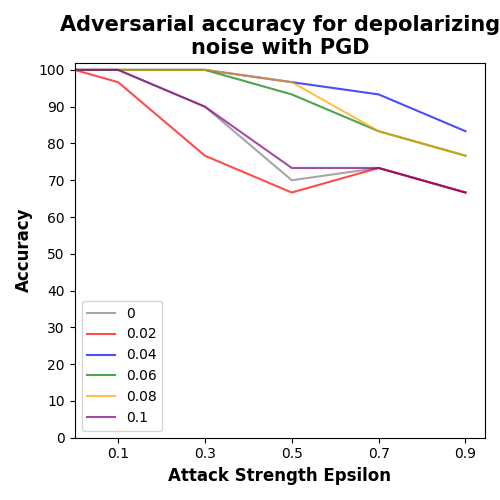
\includegraphics[width=\linewidth]{figures/evaluation_results/iris/pqc/figures/depolarizing-pgd.png}
      \subcaption{Depolarizing noise model's \ac{pgd} adversarial accuracy.}
      \label{fig:iris12}
  \end{subfigure}
  \caption{Depolarizing noise models' accuracy on the adversarial Iris test dataset.}
  \label{fig:iris-1112}
\end{figure} \

\begin{figure}[!h]
  \centering

  \begin{subfigure}{0.45\textwidth}
      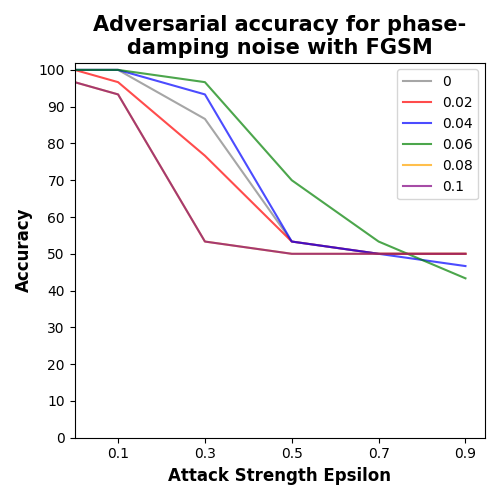
\includegraphics[width=\linewidth]{figures/evaluation_results/iris/pqc/figures/phase-damping-fgsm.png}
      \subcaption{Phase Damping noise model's \ac{fgsm} adversarial accuracy.}
      \label{fig:iris13}
  \end{subfigure} \qquad
  \begin{subfigure}{0.45\textwidth}
      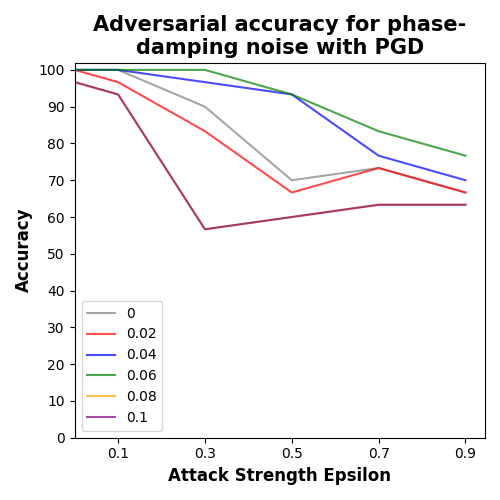
\includegraphics[width=\linewidth]{figures/evaluation_results/iris/pqc/figures/phase-damping-pgd.png}
      \subcaption{Phase Damping noise model's \ac{pgd} adversarial accuracy.}
      \label{fig:iris14}
  \end{subfigure}
  \caption{Phase damping models' accuracy on the adversarial Iris test dataset.}
  \label{fig:iris-1314}
\end{figure} \

\begin{figure}[!h]
  \centering

  \begin{subfigure}{0.45\textwidth}
      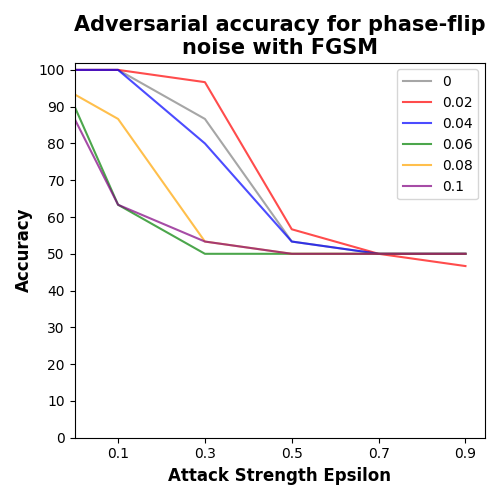
\includegraphics[width=\linewidth]{figures/evaluation_results/iris/pqc/figures/phase-flip-fgsm.png}
      \subcaption{Phase-Flip noise model's \ac{fgsm} adversarial accuracy.}
      \label{fig:iris15}
  \end{subfigure} \qquad
  \begin{subfigure}{0.45\textwidth}
      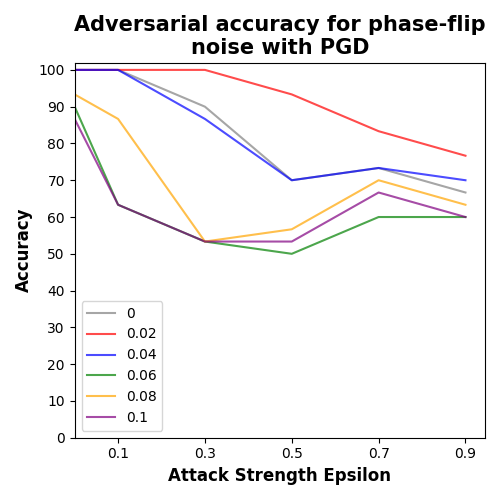
\includegraphics[width=\linewidth]{figures/evaluation_results/iris/pqc/figures/phase-flip-pgd.png}
      \subcaption{Phase-Flip noise model's \ac{pgd} adversarial accuracy.}
      \label{fig:iris16}
  \end{subfigure}

  \caption{Phase-Flip noise models' accuracy on the adversarial Iris test dataset.}
  \label{fig:iris-1516}
\end{figure} \

Amplitude damping works worse than baseline, no relation between noise
probability and adv accuracy. \

bit-flip, some models perform better than baseline but no relationship
between noise probability and adv accuracy can be found. \

\section{\acl{pid} Dataset}\label{section:diabetes-eval} \

\subsection{Noisy Models Accuracy}\label{subsection:diabetes-noisy-acc} \

\subsection{Adversarial Accuracy}\label{subsection:diabetes-adv-acc} \

\subsection{Noisy Models Adversarial Accuracy}\label{subsection:diabetes-noisy-adv-acc} \

\section{Breast Cancer Dataset}\label{section:breast-cancer-eval} \

\subsection{Noisy Models Accuracy}\label{subsection:breast-cancer-noisy-acc} \

\subsection{Adversarial Accuracy}\label{subsection:breast-cancer-adv-acc} \

\subsection{Noisy Models Adversarial Accuracy}\label{subsection:breast-cancer-noisy-adv-acc} \

\section{Plus-Minus Dataset}\label{section:plus-minus-eval} \

\subsection{Noisy Models Accuracy}\label{subsection:plus-minus-noisy-acc} \

\subsection{Adversarial Accuracy}\label{subsection:plus-minus-adv-acc} \

\subsection{Noisy Models Adversarial Accuracy}\label{subsection:plus-minus-noisy-adv-acc} \

\subsection{Discussion}\label{subsection:discussion} \

Iris dataset might be too simple on clean dataset.

Coherent noise might just work as a bias term on the clean dataset.(?) \


1.	Explain why decoherent noise is used and not coherent. \

  a. Coherent noise will probably just shift the bias. \

  b. Coherent noise might add too much noise (quadratic growth). \

  c. True random noise is required to improve generalization. \

% TODO: Do an experiment implementing coherent noise to prove this claim.
% Use https://pennylane.ai/qml/demos/tutorial_variational_classifier/ - circuit-centric quantum classifier ansatz

\section{Variational Quantum Algorithm Model Accuracy}\label{section:vqa_accuracy} \

% TODO: State the result of training QVC with regards to the chosen datasets.
% TODO: Compare to paper and state why they might be valid results.

\section{Variational Quantum Algorithm Model Adversarial Accuracy}\label{section:vqa_adversarial_accuracy} \

% TODO: Present results per dataset of the different attacks and attack strengths